\documentclass[10pt]{article}
\usepackage[utf8]{inputenc}
\usepackage[english]{babel}
\usepackage[font=small,labelfont=bf]{caption}
\usepackage{geometry}
\usepackage[sort&compress, numbers]{natbib}
\usepackage{pxfonts}
\usepackage{graphicx}
\usepackage{setspace}
\usepackage{hyperref}
\usepackage{lineno}

% supplemental tables
\newcommand{\questions}{S1}
\newcommand{\topics}{S2}

% supplemental figures
\newcommand{\individualKnowledgeMapsA}{S1}
\newcommand{\individualKnowledgeMapsB}{S2}
\newcommand{\individualKnowledgeMapsC}{S3}
\newcommand{\individualLearningMapsA}{S4}
\newcommand{\individualLearningMapsB}{S5}

% simple command for inline comments
\newcommand{\comment}[1]{}

\doublespacing
\linenumbers

%\title{Text embedding models reveal high-resolution insights into conceptual
%knowledge and learning from short multiple-choice quizzes}
\title{A geometric framework for capturing high-resolution insights into
conceptual knowledge and learning in classroom-like settings}

\author{Paxton C. Fitzpatrick\textsuperscript{1},
Andrew C. Heusser\textsuperscript{1, 2}, and Jeremy R.
Manning\textsuperscript{1, *}\\\small{\textsuperscript{1}Department of Psychological and Brain Sciences}\\\small{Dartmouth College, Hanover, NH 03755, USA}\\\small{\textsuperscript{2}Akili Interactive Labs}\\\small{Boston, MA 02110, USA}\\\small{\textsuperscript{*}Corresponding author:
Jeremy.R.Manning@Dartmouth.edu}}

\date{}

\begin{document}
\maketitle

\begin{abstract}\noindent We develop a mathematical framework, based on natural language
processing models, for tracking and characterizing the acquisition of
conceptual knowledge in real-world educational contexts. Our approach embeds
course content in a high-dimensional
conceptual space, where nearby coordinates reflect similar or related
concepts. We test our approach using behavioral data from participants who
watched two lecture videos from the Khan Academy platform, interleaved
between three short multiple-choice quizzes. We applied our
framework to the videos' transcripts and the text of the quiz questions to
quantify the conceptual content presented in each moment of video and knowledge probed by each quiz question. We used
these embeddings, along with participants' quiz responses, to track how the
learners' knowledge changed after watching each video. Our findings demonstrate how a
small set of quiz questions may be used to obtain rich and meaningful 
high-resolution insights into individual students' knowledge, and how it
changes over time as they learn.

\textbf{Keywords: education, learning, knowledge, concepts, natural language processing}

\end{abstract}


\section*{Introduction}

Suppose that a teacher had access to a complete ``map'' of everything a
student knew. Defining what such a map might even look like, let alone how it
might be constructed or filled in, is itself a non-trivial problem. But if a
teacher \textit{were} to gain access to such a map, how might it change their
ability to teach that student? Perhaps they might start by checking how well the
student knew the to-be-learned information already, or how much they knew about
related concepts. For some students, they could potentially optimize their
teaching efforts to maximize efficiency by focusing primarily on not-yet-known
content. For other students (or other content areas), it might be more
effective to optimize for direct connections between already known content and
new material. Observing how the student's knowledge changed over time,
in response to their teaching, could also help to guide the teacher towards
the most effective strategy for that individual student.

Designing and building procedures and tools for mapping out knowledge touches
on deep questions about what it means to learn. For example, how do we acquire
conceptual knowledge? Memorizing course lectures or textbook chapters by rote
can lead to the superficial \textit{appearance} of understanding the underlying
content, but achieving true conceptual understanding seems to require something
deeper and richer. Does conceptual understanding entail connecting newly
acquired information to the scaffolding of one's existing knowledge or
experience~\citep{BlayEtal06,CaraMaho03, ConsEtal16, DeacEtal04, SimoEtal04}?
Or weaving a lecture's atomic elements (e.g., its component words) into a
structured network that describes how those individual elements are related?
Conceptual understanding could also involve building a mental model that
transcends the meanings of those individual atomic elements by reflecting the
deeper meaning underlying the gestalt whole~\citep{Kint70, Macl05, ScotEtal07}.

The difference between ``understanding'' and ``memorizing,'' as framed by
researchers in education, cognitive psychology, and cognitive
neuroscience~\citep[e.g.,][]{Kato40, Gall00, ScotEtal07, HallGree08, Macl05} has
profound analogs in the fields of natural language processing and natural
language understanding. For example, considering the raw contents of a document
(e.g., its constituent symbols, letters, and words) might provide some
information about what the document is about, just as memorizing a passage
might provide some ability to answer simple questions about it~\citep[e.g., whether
it contains words related to furniture versus physics;][]{LandDuma97,
BleiEtal03, BleiLaff06}. However, modern natural language processing
models~\citep[e.g.,][]{MikoEtal13a, CerEtal18, BrowEtal20} also attempt to
capture the deeper meaning \textit{underlying} those atomic elements. These
models consider not only the co-occurrences of those elements within and across
documents, but also patterns in how those elements appear across different
scales (e.g., sentences, paragraphs, chapters, etc.), the temporal and
grammatical properties of the elements, and other high-level characteristics of
how they are used~\citep{Mann20, Mann21a}. According to these models, the deep
conceptual meaning of a document may be captured by a feature vector in a
high-dimensional representation space, where nearby vectors reflect
conceptually related documents. A model that succeeds at capturing an analog of
``understanding'' is able to assign nearby feature vectors to two conceptually
related documents, \textit{even when the words contained in those documents
have very little overlap}.

Given these insights, what form might the representation of the sum total of a
person's knowledge take? First, we might require a means of systematically
describing or representing the nearly infinite set of possible things a person
could know. Second, we might want to account for potential associations between
different concepts. For example, the concepts of ``fish'' and ``water'' might
be associated in the sense that fish live in water. Third, knowledge may have a
critical dependency structure, such that knowing about a particular concept
might require first knowing about a set of other concepts. For example,
understanding the concept of a fish swimming in water first requires
understanding what fish and water \textit{are}. Fourth, as we learn, our
``current state of knowledge'' should change accordingly. Learning new concepts
should both update our characterizations of ``what is known'' and also
unlock any now-satisfied dependencies of those newly learned concepts so that
they are ``tagged'' as available for future learning.
% TODO: is the second half of this paragraph relevant to this paper??

Here we develop a framework for modeling how knowledge is acquired during
learning. The central idea is to use text embedding models to define the
coordinate systems of two maps: (a) a \textit{knowledge map} that describes the
extent to which each concept is currently known and (b) a \textit{learning map}
that describes changes in knowledge over time. Each location on these maps
represents a single concept, and the maps' geometries are defined such that
related concepts are located nearby in space. We use this framework to analyze
and interpret behavioral data collected from an experiment that had
participants watch and answer multiple-choice questions about a series of
recorded course lectures.

Our primary research goal is to advance our understanding of what it means to
acquire deep real-world conceptual knowledge. Traditional laboratory approaches
to studying learning and memory (e.g., list learning studies) often draw little
distinction between memorization and understanding. Instead, these studies
typically focus on whether information is effectively encoded or retrieved,
rather than whether the information is \textit{understood}. Approaches to
studying conceptual learning, such as category learning experiments, can start
to investigate the distinction between memorization and understanding, often by
training participants to distinguish arbitrary or random features in otherwise
meaningless categorized stimuli. However the objective of real-world training,
or learning from life experiences more generally, is often to develop new
knowledge that may be applied in \textit{useful} ways in the future. In this
sense, the gap between modern learning theories and modern pedagogical
approaches and classroom learning strategies is enormous: most of our theories
about \textit{how} people learn are inspired by experimental paradigms and
models that have only peripheral relevance to the kinds of learning that
students and teachers actually seek \citep{Macl05, HallGree08}. To help bridge this gap, our study uses
course materials from real online courses to inform, fit, and test models of
real-world conceptual learning. We also provide a ``proof of concept''
demonstration of how our models might be used to construct ``maps'' of what
students know, and how their knowledge changes with training. In addition to
helping to visualize knowledge (and changes in knowledge), we hope that such
maps might lead to real-world tools for improving how we educate.

\section*{Results}

At its core, our main modeling approach is based around a simple assumption
that we sought to test empirically: all else being equal, knowledge about a
given concept is predictive of knowledge about similar or related concepts.
From a geometric perspective, this assumption implies that knowledge is
fundamentally ``smooth.'' In other words, as one moves through a space
representing an individual's knowledge (where similar concepts occupy nearby
coordinates), their ``level of knowledge'' should change relatively gradually
throughout that space. To begin to test this smoothness assumption, we sought
to track our participants' knowledge and how it changed over time in response
to training.

\begin{figure}[tp]
    \centering
    \includegraphics[width=\textwidth]{figs/experiment}

    \caption{\textbf{Experimental paradigm.} Participants alternate between
    answering 13-question multiple-choice quizzes and watching two Khan Academy
    lectures. Each quiz contains a mix of 5 questions about lecture 1, 5
    questions about lecture 2, and 3 questions about general physics knowledge. The
    specific questions reflected on each quiz, and the orders of each quiz's
    questions, were randomized across participants.}

    \label{fig:experiment}
\end{figure}

We asked participants in our study to answer questions from several multiple-choice
quizzes and watch two lecture videos from the Khan Academy platform
(Fig.~\ref{fig:experiment}). The first lecture video, entitled \textit{Four
Fundamental Forces}, discussed the four fundamental forces in physics: gravity,
strong and weak interactions, and electromagnetism. The second,
entitled \textit{Birth of Stars}, provided an overview of our current
understanding of how stars form. We selected these lessons to be (a) accessible
to a broad audience, i.e., requiring minimal prerequisite knowledge to understand;
(b) conceptually related to each other, i.e., covering at least \textit{some}
similar or overlapping content; and (c) largely independent of each other, i.e., focused
on sufficiently different material that understanding one did not require having seen
the other. Thus, the two videos we selected are introductory, high-level lectures that both 
belong to Khan Academy's ``Cosmology and Astronomy" course domain, but come from
different lecture series (``Scale of the Universe" and ``Stars, Black Holes, and Galaxies" 
for the first and second lectures, respectively). 

We also wrote a set of
multiple-choice quiz questions that would enable us to test participants'
knowledge about each individual lecture, as well as related content not
specifically presented in either video ( see Tab.~\questions). Participants answered
questions randomly drawn from each content area (lecture 1, lecture 2, and
general physics knowledge) across each of three quizzes. Quiz 1 was intended to
assessed participants' ``baseline" knowledge before training, quiz 2 assessed knowledge
after watching the \textit{Four Fundamental Forces} video (i.e., lecture 1),
and quiz 3 assessed knowledge after watching the \textit{Birth of Stars} video
(i.e., lecture 2).

We trained a topic model \citep{BleiEtal03} using sliding windows of text from the two
lectures' transcripts (see \hyperref[subsec:topic-modeling]{\textit{Constructing text embeddings of multiple
lectures and questions}}). We also used the same model (i.e., trained on the
videos' transcripts) to embed the text of each question in our pool. This
yielded, for each second of each video, and for each question, a single
15-dimensional topic vector---i.e., a coordinate in a text embedding space
(Fig.~\ref{fig:sliding-windows}). Intuitively, each dimension of the embedding
space corresponds to a ``theme'' or ``topic'' reflected in some part(s) of the
videos (Tab.~\topics), and the coordinates in embedding space denote the blend
of themes reflected by a particular excerpt of text (e.g., from part of a
video's transcript, from a question, etc.).

\begin{figure}[tp]
    \centering
    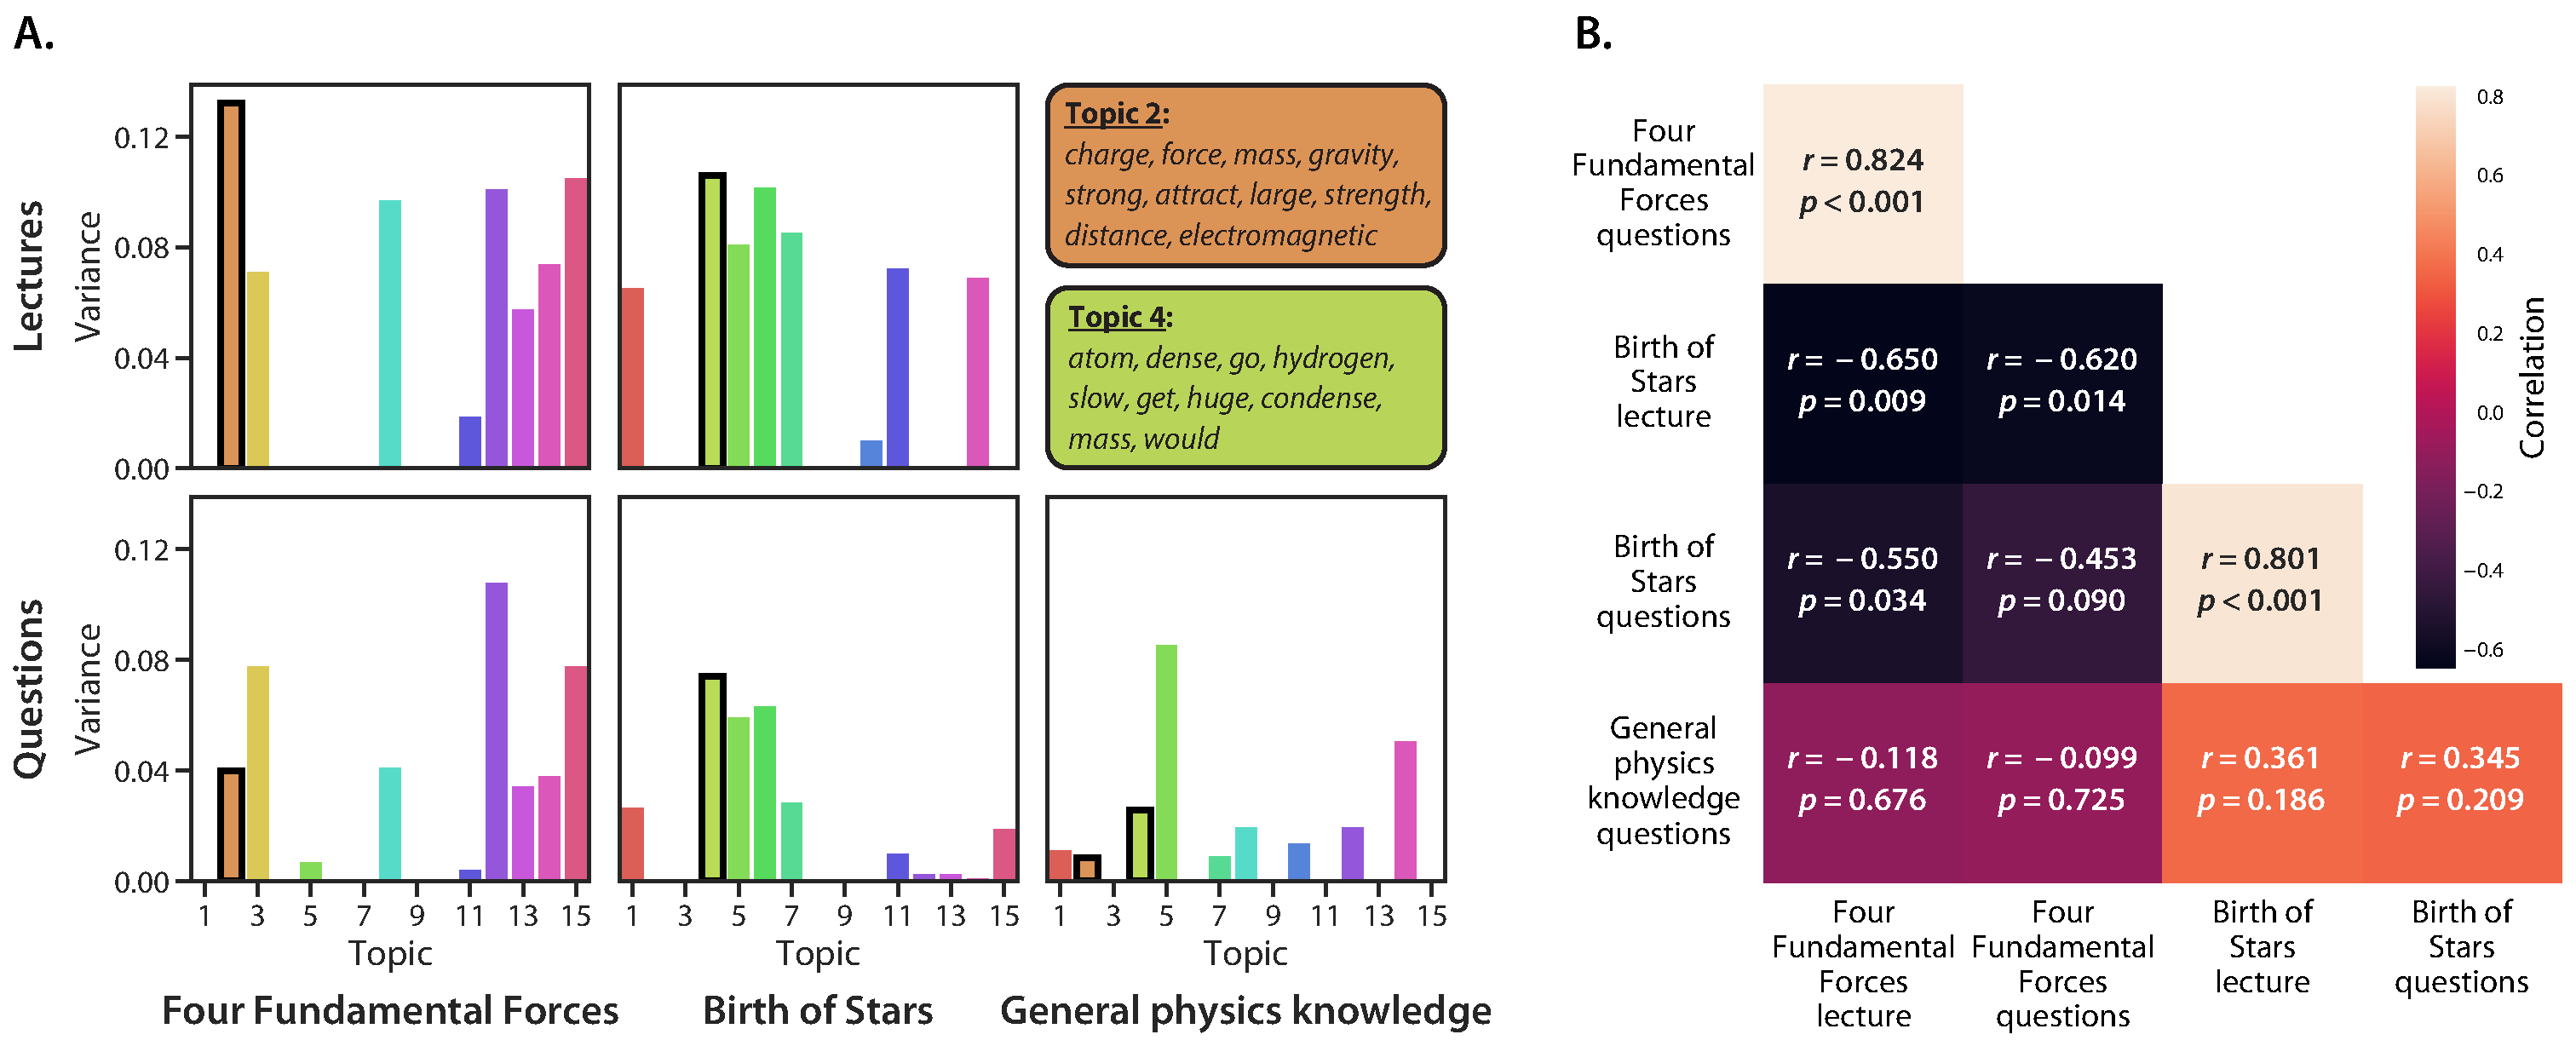
\includegraphics[width=0.7\textwidth]{figs/active-topics}

\caption{\textbf{Lecture and question topic overlap.} The bar plots display the
variability in topic weights across lecture timepoints (top panels) and
questions (bottom panels); colors denote topics. The top-weighted words from
the most ``expressive'' (i.e., variable across observations) topic from each
lecture are displayed in the upper right (orange: topic 2; yellow-green: topic
4). The top-weighted words from the full set of topics may be found in
Table~\topics.}

    \label{fig:topics}
\end{figure}


Given that we trained the text embedding model using the video transcripts, we
wondered whether the questions that were (ostensibly, by design) ``about'' the
content of each lecture would ``match up'' correctly with the lectures. In
other words, we hoped that the text embeddings would capture something about
the deeper conceptual content of the lectures, beyond surface details such as
exact wording choices. If so, when we embed \textit{new} text outside of the
model's training set, we should see a correspondance between the embeddings of
the training data (i.e., snippets of text from the lectures' transcripts) and
other text that reflects related concepts (e.g., questions \textit{about} each
lecture). Further, although the content from any given moment from a lecture
might stray from the average content (across all timepoints), we hoped that
\textit{variability} in each topic's expression over timepoints within a
lecture would match up with the variability in topic expressions for questions
about that lecture. Intuitively, the variability in the expression of a given
topic relates to how much ``information''~\citep{Fish22} the lecture (or
questions) reflect about that topic. When we compared the variability in topic
weights across each lecture's timepoints with the variability in topic weights
across each question set, we found a strong correspondence
(Fig.~\ref{fig:topics}). The most variable topics from the \textit{Four
Fundamental Forces} lecture, and questions about that lecture, are 2, 3, 8, 12,
13, 14, and 15. The most variable topics from the \textit{Birth of Stars}
lecture, and questions about that lecture, are 1, 4, 5, 6, and 7. This strong
overlap between the lectures and questions specifically about each lecture
indicates that the topic model captures some of the underlying conceptual
content.


\begin{figure}[tp]
    \centering
    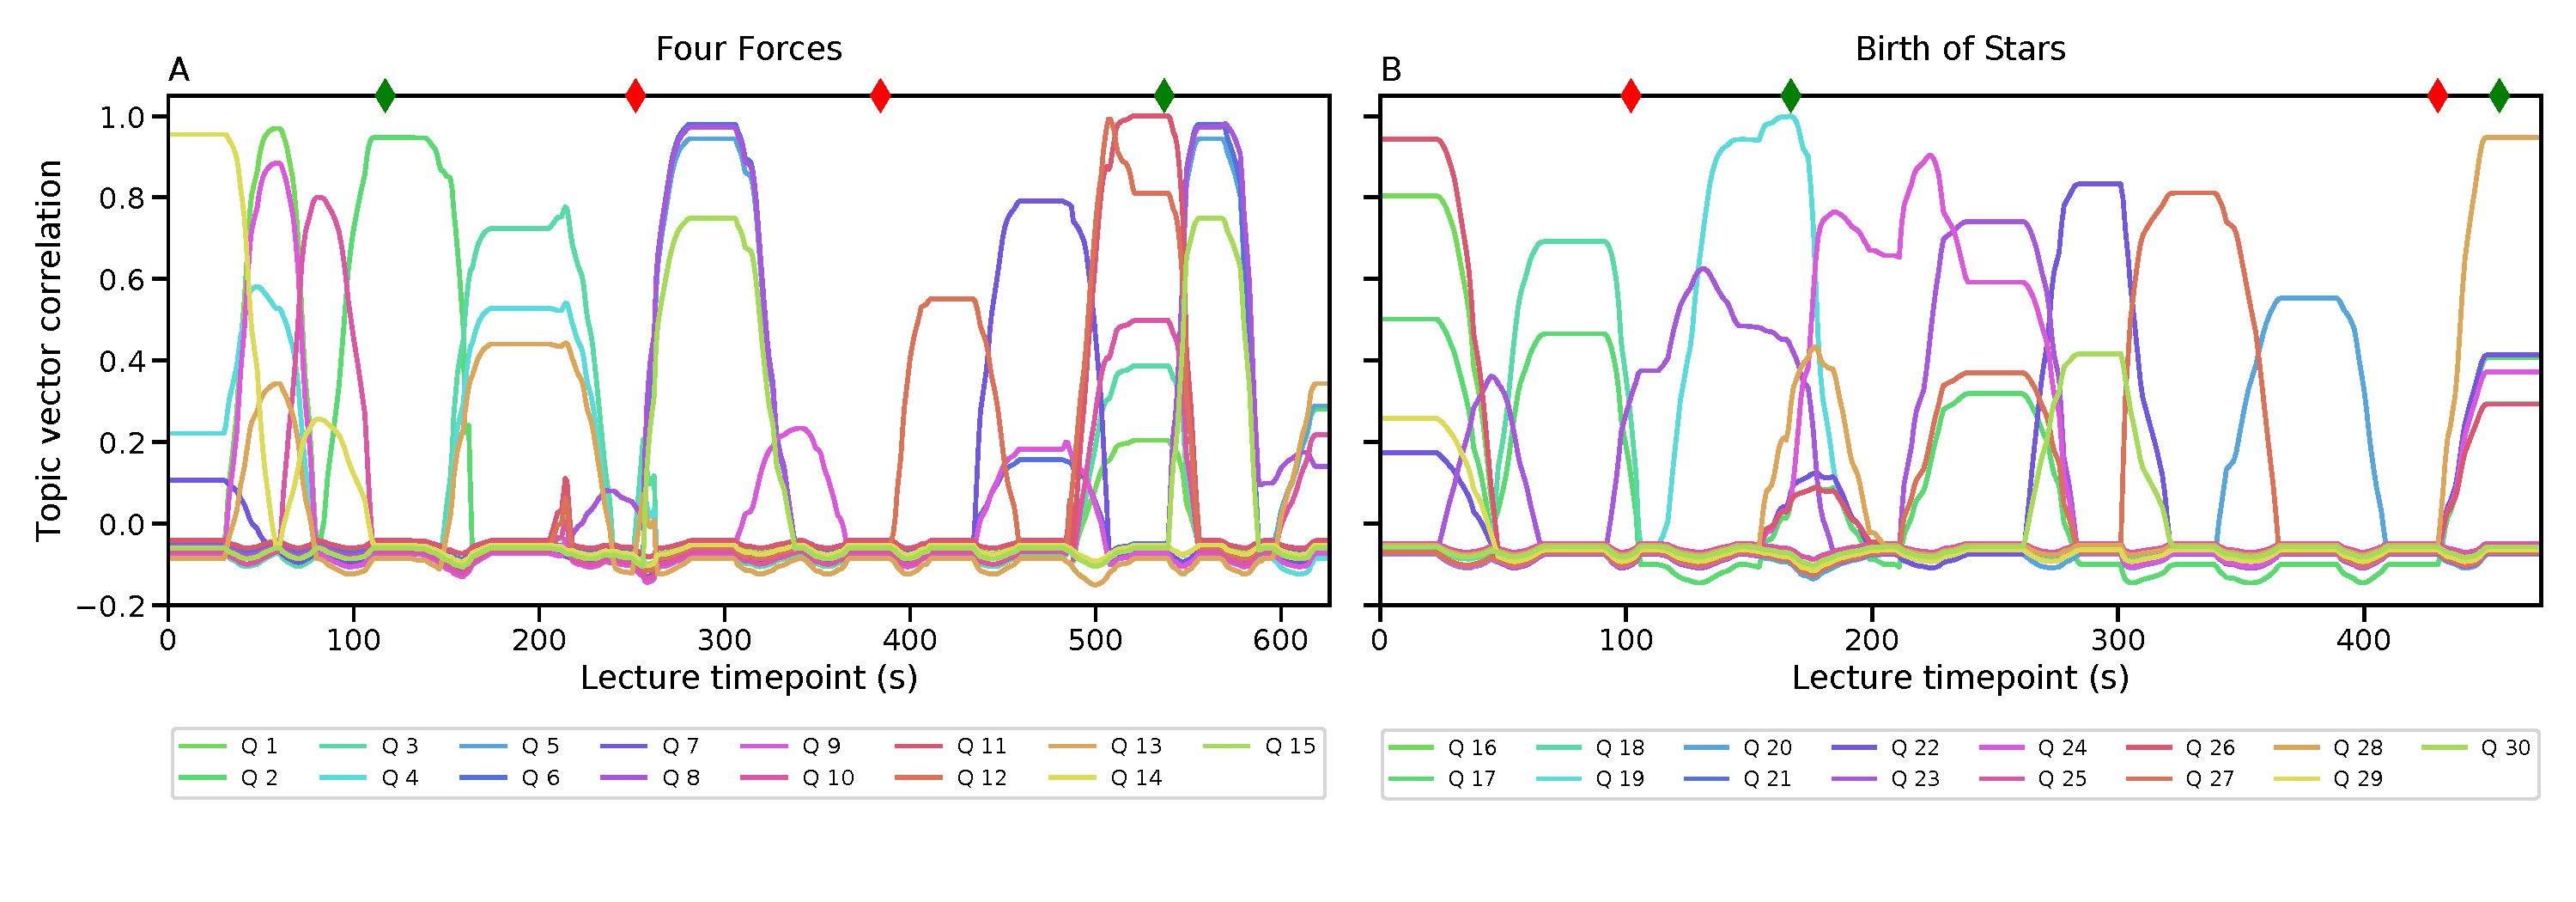
\includegraphics[width=\textwidth]{figs/lecture-question-similarity}

    \caption{\textbf{Which parts of each lecture are captured by each
    question?} Each panel displays timeseries plots showing how each question's
    topic vector correlates with each video timepoint's topic vector (Panel
    \textbf{A.}: correlations for the \textit{Four Fundamental Forces} lecture
    and associated questions; Panel \textbf{B.}: correlations for the
    \textit{Birth of Stars} lecture and associated questions). The colors denote
    question identities. The diamonds in each panel denote the moment of peak
    correlation between the indicated questions, in the indicated lectures. The
    associated questions' text, and snippets of the lectures' transcripts in
    the best-matching sliding windows, are displayed at the bottom of the
    figure.}

    \label{fig:question-correlations}
\end{figure}

Although a single lecture may be organized around a single broad theme at a
coarse scale, at a finer scale each moment of a lecture typically covers a
narrower range of content. We wondered whether a text embedding model trained
on the lectures' transcripts might capture some of this finer scale content.
For example, if a particular question asks about the content from one small
part of a lecture, we wondered whether our text embedding model could be used
to automatically identify the ``matching'' moment(s) in the lecture. When we
correlated each question's topic vector with the topic vectors for each second
of the lectures, we found some evidence that each question is temporally
specific (Fig.~\ref{fig:question-correlations}). In particular, most questions'
topic vectors were maximally correlated with a well-defined (and relatively
narrow) range of timepoints from their corresponding lectures, and the
correlations fell off sharply outside of that range. We also examined the
best-matching intervals for each question qualitatively by comparing the text
of the question to the text of the most-correlated parts of the lectures.
Despite that the questions were excluded from the text embedding model's
training set, in general we found (through manual inspection) a close
correspondence between the conceptual content that each question covered and
the content covered by the best-matching moments of the lectures. Two
representative examples are shown at the bottom of
Figure~\ref{fig:question-correlations}.

The ability to quantify how much each question is ``asking about'' the content
from each moment of the lectures could enable high-resolution insights into
participants' knowledge. Traditional approaches to estimating how much a
student ``knows'' about the content of a given lecture entail computing the
proportion of correctly answered questions. But if two students receive
identical scores on an exam, might our modeling framework help us to gain more
nuanced insights into the \textit{specific} content that each student has
mastered (or failed to master)? For example, a student who misses three
questions that were all about the same concept (e.g., concept $A$) will have
gotten the same \textit{proportion} of questions correct as another student who
missed three questions about three \textit{different} concepts (e.g., $A$, $B$,
and $C$). But if we wanted to fill in the ``gaps'' in the two students'
understandings, we might do well to focus on concept $A$ for the first student,
but to also add in materials pertaining to concepts $B$ and $C$ for the second
student.

We developed a simple formula (Eqn.~\ref{eqn:prop}) for using a participant's
responses to a small set of multiple-choice questions to estimate how much the
participant ``knows'' about the concept reflected by any arbitrary coordinate,
$x$, in text embedding space (e.g., the content reflected by any moment in a
lecture they had watched; see \textit{Estimating dynamic knowledge traces}).
Essentially, the estimated knowledge at the coordinate is given by the weighted
average proportion of quiz questions the participant answered correctly, where
the weights reflect how much each question is ``about'' the content at $x$.
When we apply this approach to estimate the participant's knowledge about the
content presented in each moment of each lecture, we can obtain a detailed
timecourse describing how much ``knowledge'' the participant has about any part
of the lecture. As shown in Figure~\ref{fig:knowledge-timeseries}, we can also
apply this approach separately for the questions from each quiz the
participants took throughout the experiment. From just 13 questions per quiz,
we obtain a high-resolution snapshot (at the time each quiz was taken) of what
the participants knew about any moment's content, from either of the two
lectures they watched (comprising a total of 1106 samples across the two
lectures).


\begin{figure}[tp]
    \centering
    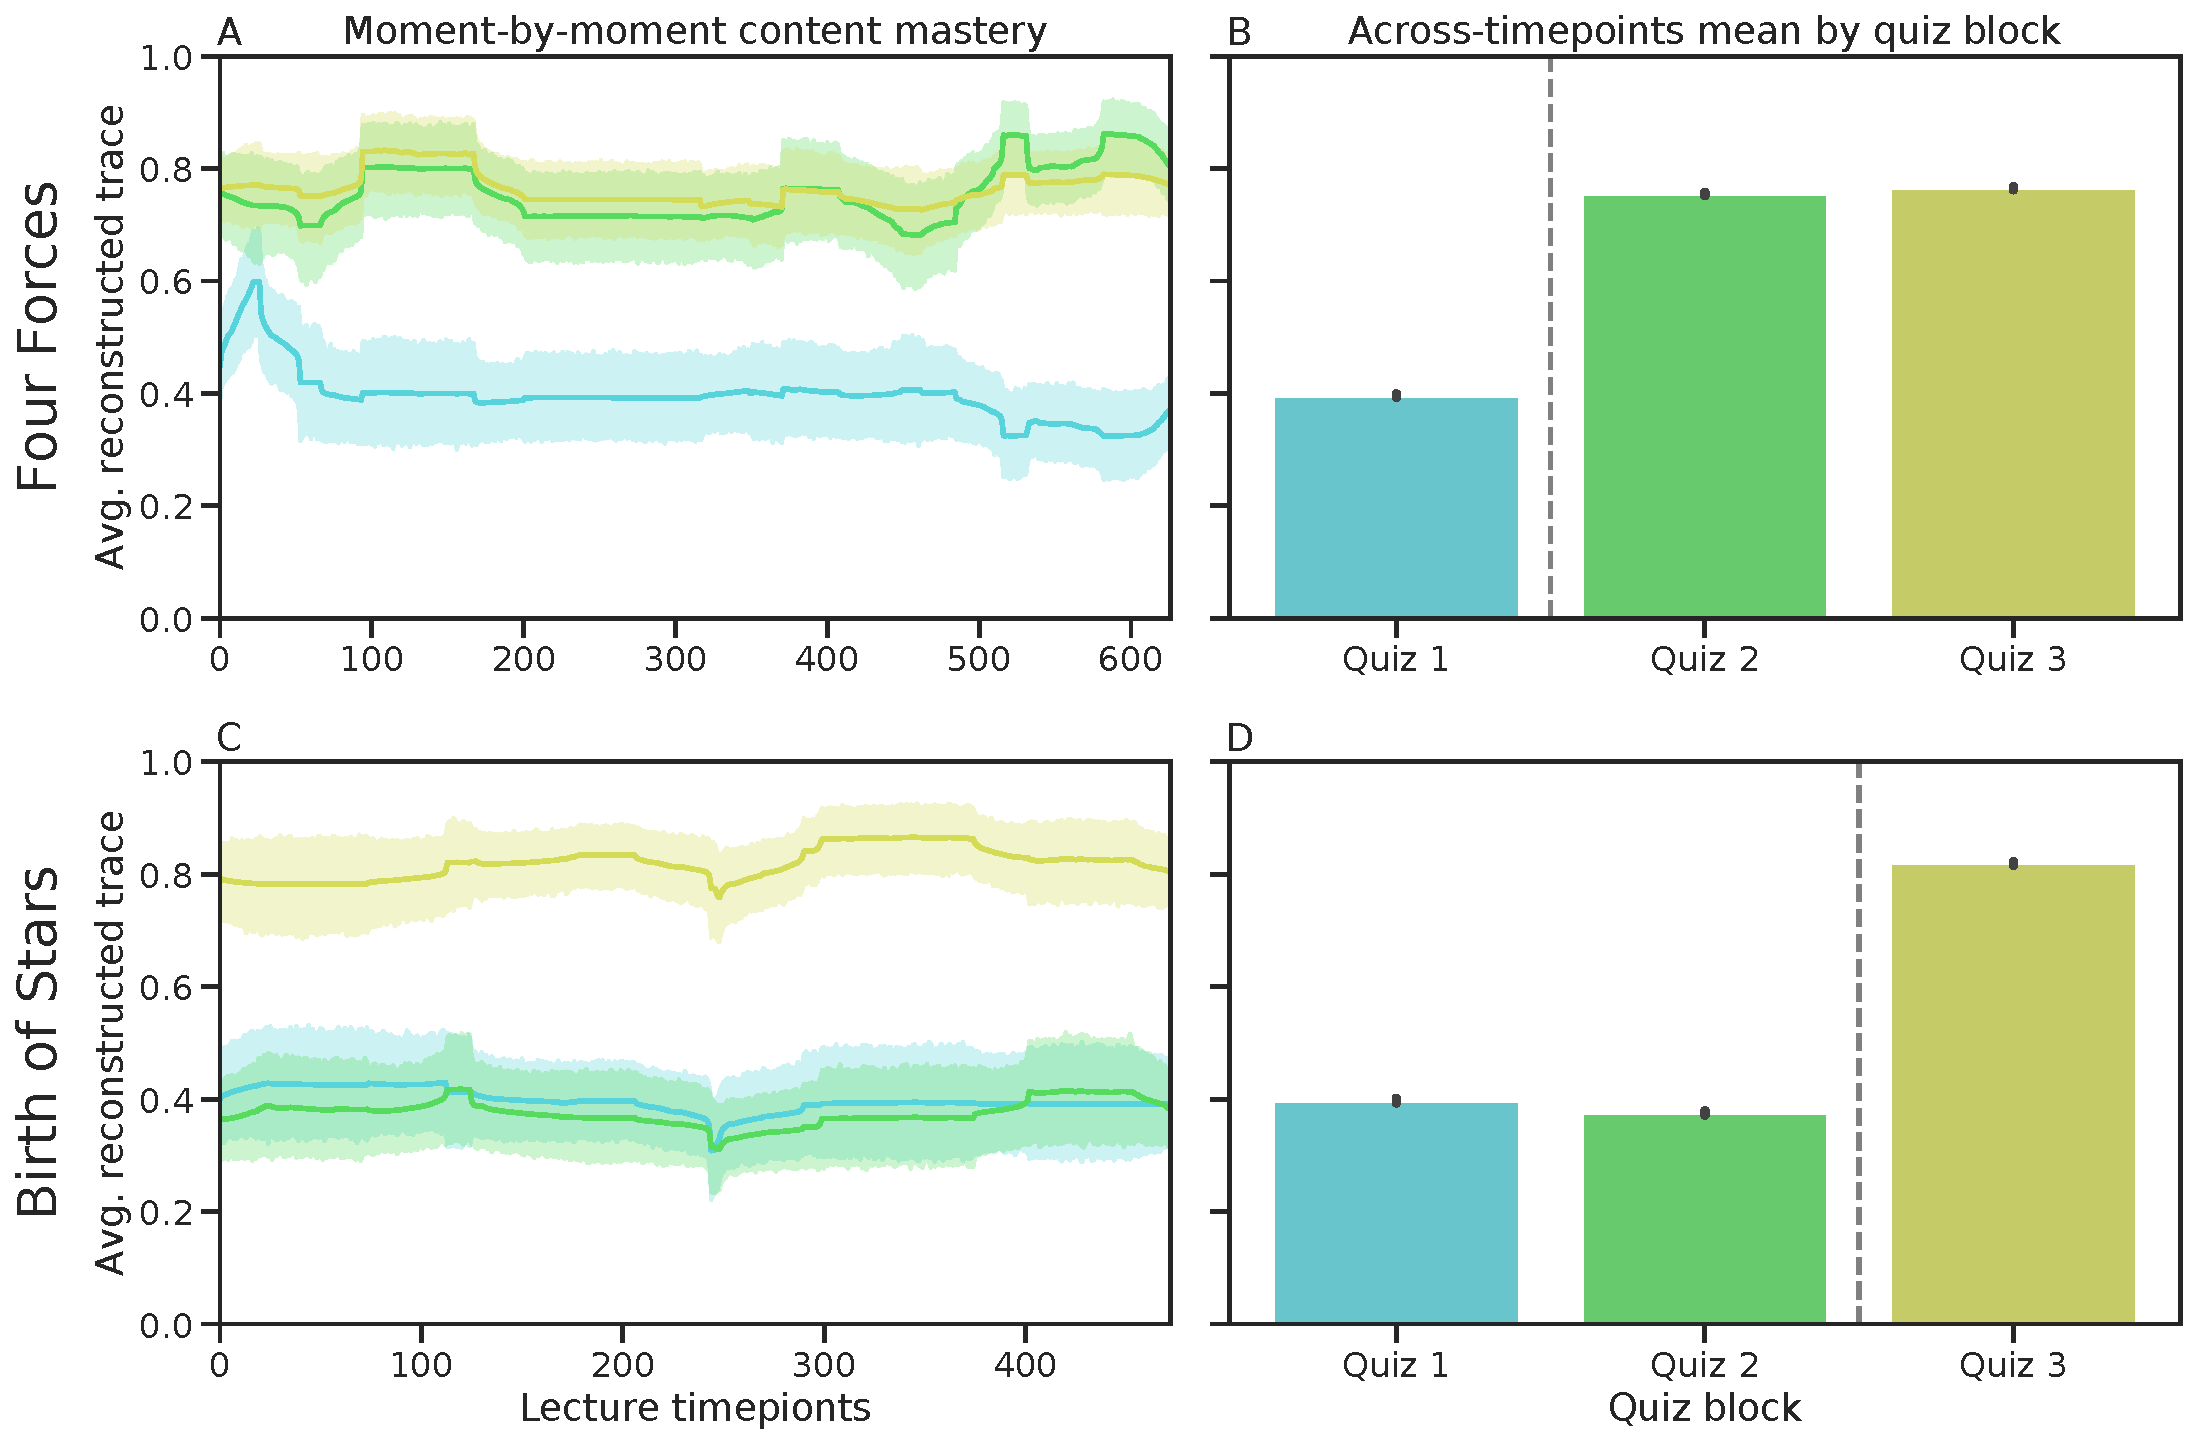
\includegraphics[width=0.7\textwidth]{figs/content-mastery}

    \caption{\textbf{Estimating moment-by-moment knowledge acquisition.}
    \textbf{A. Moment-by-moment knowledge about the \textit{Four Fundamental
    Forces}}. Each trace displays the weighted proportion of correctly answered
    questions about the content reflected in each moment of the lecture (see
    \textit{Estimating dynamic knowledge traces}), using responses from one
    quiz (color). The traces are averaged across participants. \textbf{B.
    Average estimated knowledge about the \textbf{Four Fundamental Forces}.}
    Each bar displays the across-timepoint average knowledge, estimated using
    the responses to one quiz's questions. \textbf{C. Moment-by-moment
    knowledge about the \textit{Birth of Stars}}. The panel is in the same
    format as Panel A, but here the knowledge estimates are for the
    moment-by-moment content of the \textit{Birth of Stars} lecture. \textbf{D.
    Average estimated knowledge about the \textit{Birth of Stars}.} The panel
    is in the same format as Panel B, but here the knowledge estimates are for
    the content of the \textit{Birth of Stars} lecture. All panels: error
    ribbons and error bars denote 95\% confidence intervals, estimated across
    participants.}

    \label{fig:knowledge-timeseries}
\end{figure}

Of course, even though the timecourses in
Figure~\ref{fig:knowledge-timeseries}A and C provide detailed
\textit{estimates} about participants' knowlege, those estimates are only
\textit{useful} to the extent that they accurately reflect what participants
actually know. As one sanity check, we anticipated that the knowledge estimates
should show a content-specific ``boost'' in participants' knowledge after
watching each lecture. In other words, if participants learn about each
lecture's content when they watch each lecture, the knowledge estimates should
reflect that. After watching the \textit{Four Fundamental Forces} lecture,
participants should show more knowledge for the content of that lecture than
they had before, and that knowledge should persist for the remainder of the
experiment. Specifically, knowledge about that lecture's content should be
relatively low when estimated using Quiz 1 responses, but should increase when
estimated using Quiz 2 or 3 responses (Fig.~\ref{fig:knowledge-timeseries}B).
Indeed, we found that participants' estimated knowledge about the content of
the \textit{Four Fundamental Forces} was substantially higher on Quiz 2 versus
Quiz 1 ($t(49) = 8.764, p < 0.001$) and on Quiz 3 versus Quiz 1 ($t(49) = 10.519, p <
0.001$). We found no reliable differences in estimated knowledge about that
lecture's content on Quiz 2 versus 3 ($t(49) = 0.160, p = 0.874$). Similarly, we
hypothesized (and subsequently confirmed) that participants should show more
estimated knowledge about the content of the \textit{Birth of Stars} lecture
after (versus before) watching it (Fig.~\ref{fig:knowledge-timeseries}D).
Specifically, since participants watched that lecture after taking Quiz 2 (but
before Quiz 3), we hypothesized that their knowledge estimates should be
relatively low on Quizzes 1 and 2, but should show a ``boost'' on Quiz 3.
Consistent with this prediction, we found no reliable differences in estimated
knowledge about the \textit{Birth of Stars} lecture content on Quizzes 1 versus
2 ($t(49) = 1.013, p = 0.316$), but the estimated knowledge was substantially higher
on Quiz 3 versus 2 ($t(49) = 10.561, p < 0.001$) and Quiz 3 versus 1 ($t(49) = 8.969, p <
0.001$).

If we are able to accurately estimate a participant's knowledge about the
content tested by a given question, the estimated knowledge should have some
predictive information about whether the participant is likely to answer the
question correctly or incorrectly. For each question in turn, for each
participant, we used Equation~\ref{eqn:prop} to estimate (using all
\textit{other} questions from the same quiz, from the same participant) the
participant's knowledge at the held-out question's embedding coordinate. For
each quiz, we grouped these estimates into two distributions: one for the
estimated knowledge at the coordinates of each \textit{correctly} answered
question, and another for the estimated knowledge at the coordinates of each
\textit{incorrectly} answered question (Fig.~\ref{fig:predictions}). We then
used independent samples $t$-tests to compare the means of these distributions
of estimated knowledge.

\begin{figure}[tp]
    \centering
    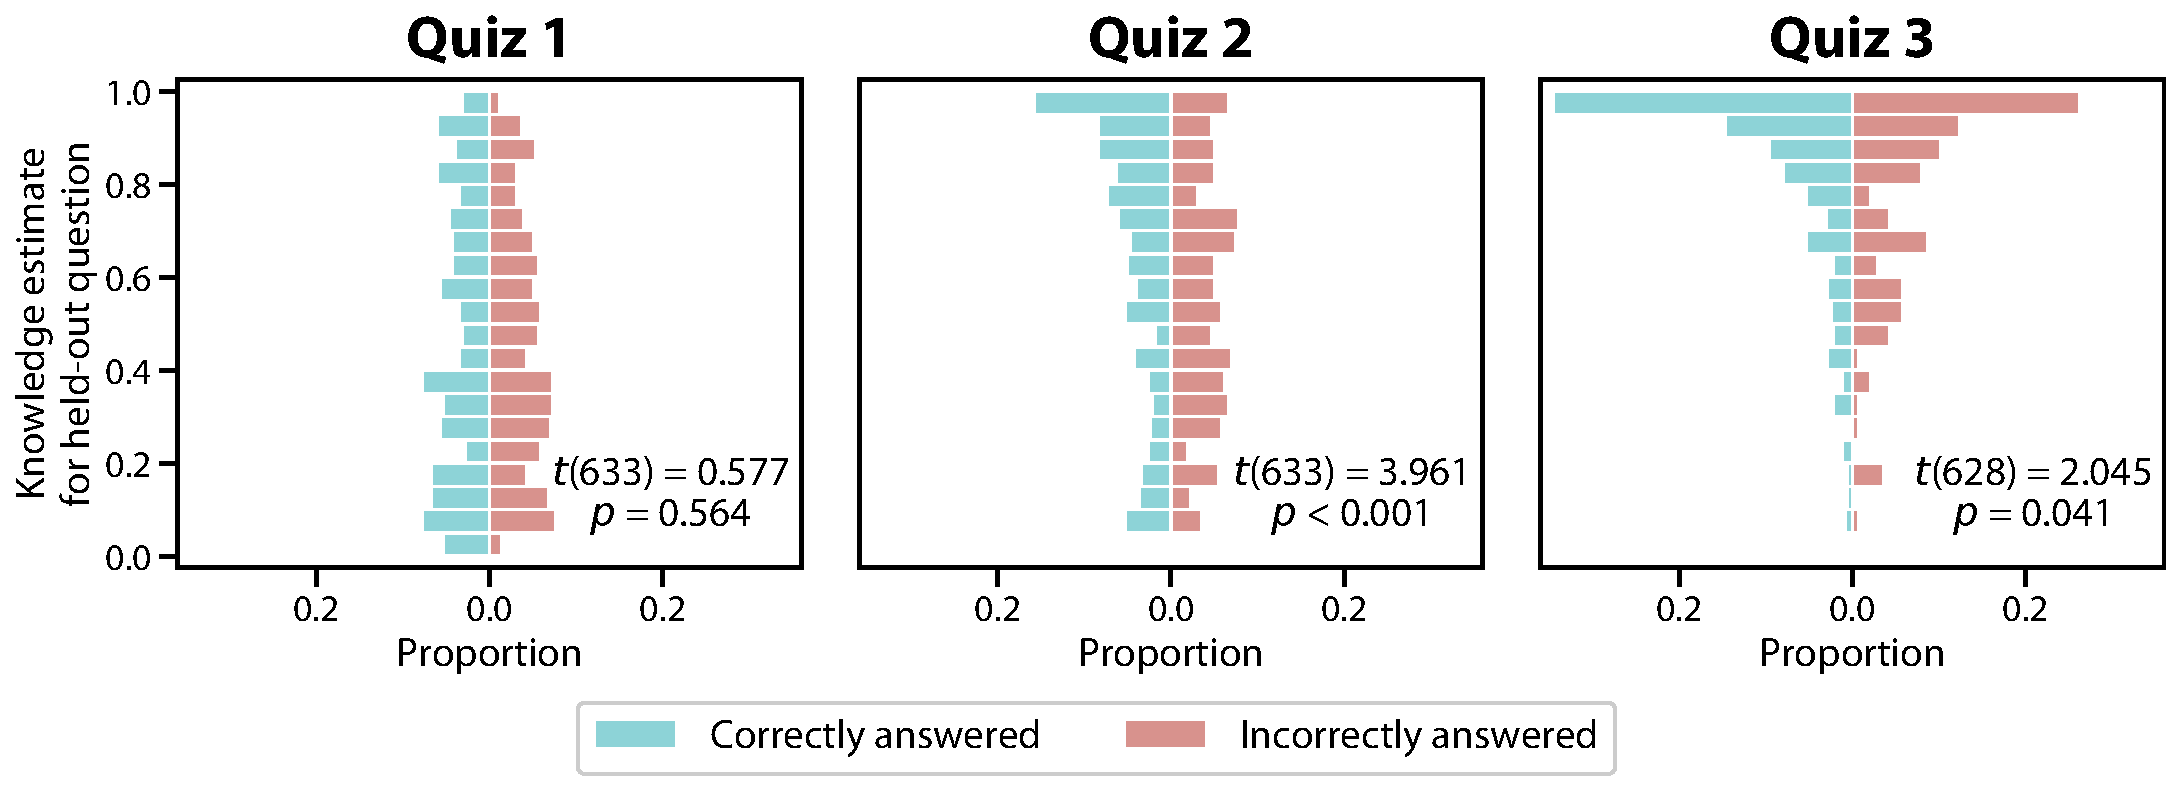
\includegraphics[width=\textwidth]{figs/held-out-question-analysis}

    \caption{\textbf{Estimating knowledge at the embedding coordinates of
    held-out questions.} Separately for each quiz (panel), we plot the
    distributions of predicted knowledge at the embedding coordinates of each
    held out correctly (blue) or incorrectly (red) answered question. The
    $t$-tests reported in each panel are between the distributions of estimated
    knowledge at the coordinates of correctly versus incorrectly answered
    held-out questions.}

    \label{fig:predictions}
\end{figure}

For the initial quizzes participants took (prior to watching either lecture),
participants' estimated knowledge tended to be low overall, and relatively
unstructured (Fig.~\ref{fig:predictions}, left panel). When we held out
individual questions and estimated their knowledge at the held-out questions'
embedding coordinates, we found no reliable differences in the estimates when
the held-out question had been correctly versus incorrectly answered ($t(633) =
0.577, p = 0.564$). After watching the first video, estimated knowledge for
held-out correctly answered questions (from the second quiz;
Fig.~\ref{fig:predictions}, middle panel) exhibited a positive shift relative
to held-out incorrectly answered questions ($t(633) = 3.961, p < 0.001$). After
watching the second video, estimated knowledge (from the third quiz;
Fig.~\ref{fig:predictions}, right panel) for \textit{all} questions exhibited a
positive shift. However, the increase in estimated knowledge for held-out
correctly answered questions was larger than for held-out incorrectly answered
questions ($t(628) = 2.045, p = 0.041$).

Knowledge estimates need not be limited to the content of the lectures. As
illustrated in Figure~\ref{fig:knowledge-maps}, our general approach to
estimating knowledge from a small number of quiz questions may be applied to
\textit{any} content, given its text embedding coordinate. To visualize how
knowledge ``spreads'' through text embedding space to content beyond the
lectures participants watched, we first fit a new topic model to the lectures'
sliding windows with $k = 100$ topics. We hoped that increasing the number of
topics from 15 to 100 might help us to generalize the knowledge predictions.
(Aside from increasing the number of topics from 15 to 100, all other
procedures and model parameters were carried over from the preceding analyses.)
As in our other analyses, we resampled each lecture's topic trajectory to 1~Hz
and also projected each question into a shared text embedding space.

\begin{figure}[tp]
    \centering
    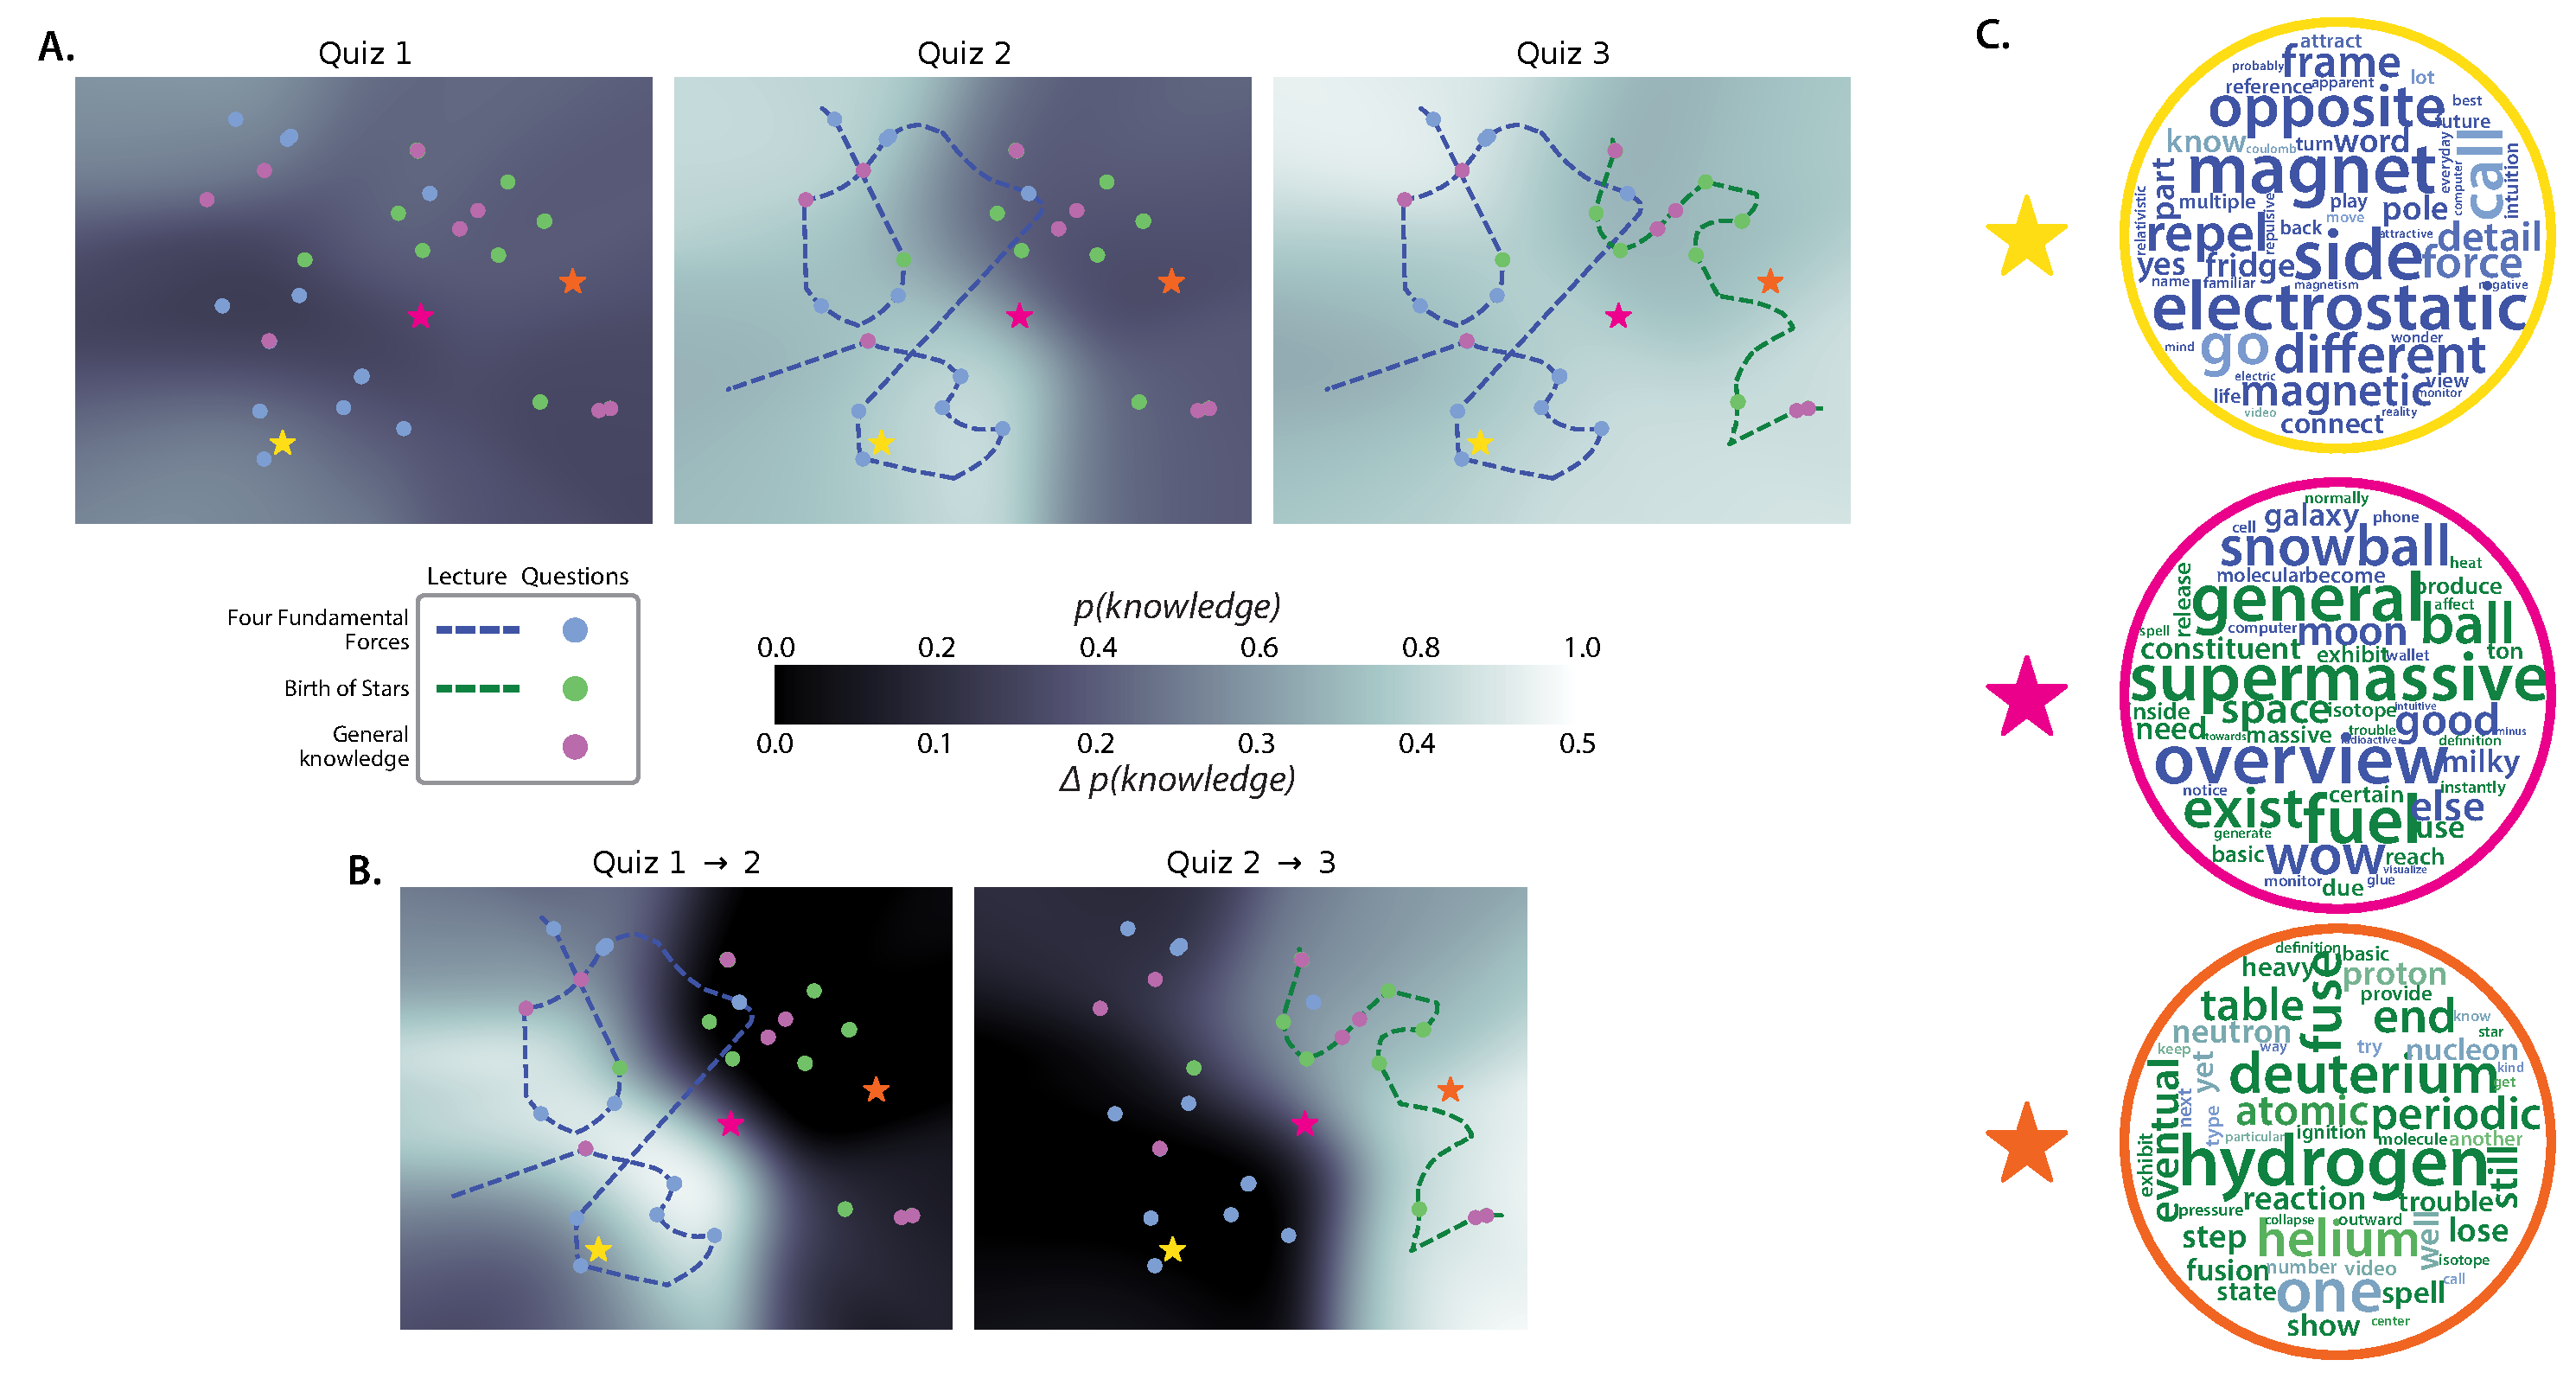
\includegraphics[width=\textwidth]{figs/knowledge_and_learning_maps}

    \caption{\textbf{Mapping out the geometry of knowledge and learning.}
    \textbf{A. Average ``knowledge maps'' estimated using each quiz.} Each map
    displays a 2D projection of the estimated knowledge about the content
    reflected by \textit{all} regions of topic space (see \textit{Creating
    knowledge and learning map visualizations}). The topic trajectories of each
    lecture and the coordinates of each question are indicated by dotted lines
    and dots. Each map reflects an average across all participants. For
    individual participants' maps, see
    Figures~\individualKnowledgeMapsA,~\individualKnowledgeMapsB,
    and~\individualKnowledgeMapsC. \textbf{B. Average ``learning maps''
    estimated between each successive pair of quizzes.} The learning maps are
    in the same general format as the knowledge maps in Panel A, but each
    coordinate in the learning maps indicates the \textit{difference} between
    the corresponding coordinates in the indicated \textit{pair} of knowledge
    maps---i.e., how much the estimated knowledge ``changed'' across the two
    quizzes. Each map reflects an average across all participants. For
    individual participants' maps, see
    Figures~\individualLearningMapsA~and~\individualLearningMapsB. \textbf{C.
    Word clouds for sampled points in topic space.} Each word cloud displays
    the relative weights of each word reflected by the blend of topics
    represented at the locations of the stars in the maps. The words' colors
    indicate how much each word is weighted on average across all timepoints'
    topic vectors in the \textit{Four Fundamental Forces} (blue) and
    \textit{Birth of Stars} (green) videos, respectively.}

    \label{fig:knowledge-maps}
    \end{figure}

We projected the resulting 100-dimensional topic vectors (for each second of
video and for each question) into a shared 2-dimensional space (see
\textit{Creating knowledge and learning map visualizations}). Next, we sampled
points evenly from a $100 \times 100$ grid of coordinates that evenly tiled a
rectangle enclosing the 2D projections of the videos and questions. We used
Equation~\ref{eqn:rbf-knowledge} to estimate participants' knowledge at each of
these 10K sampled locations, and we averaged these estimates across
participants to obtain an estimated average \textit{knowledge map}
(Fig.~\ref{fig:knowledge-maps}). Intuitively, the knowledge map constructed
from a given quiz's responses provides a visualization of how ``much''
participants know about any content expressible by the fitted text embedding
model.

Several features of the resulting knowledge maps are worth noting. The average
knowledge map estimated from Quiz 1 responses (Fig.~\ref{fig:knowledge-maps},
leftmost map) shows that participants tended to have relatively little
knowledge about any parts of the text embedding space (i.e., the shading is
relatively dark everywhere). The knowledge map estimated from Quiz 2 responses
shows a marked increase in knowledge on the left side of the map (around
roughly the same range of coordinates covered by the \textit{Four Fundamental
Forces} lecture, indicated by the dotted blue line). In other words,
participants' estimated increase in knowledge is localized to conceptual
content that is nearby (i.e., related to) the content from the lecture they
watched prior to taking Quiz 2. This localization is non-trivial: the knowledge
estimates are informed only by the embedded coordinates of the \textit{quiz
questions}, not by the embeddings of either lecture
(Eqn.~\ref{eqn:rbf-knowledge}). Finally, the knowledge map estimated from Quiz
3 responses shows a second increase in knowledge, localized to the region
surrounding the embedding of the \textit{Birth of Stars} lecture participants
watched prior to taking Quiz 3.

Another way of visualizing these content-specific increases in knowledge
(apparently driven by watching each lecture) is displayed in
Figure~\ref{fig:knowledge-maps}B. Taking the point-by-point difference between
the knowledge maps estimated from responses to a successive pair of quizzes
yields a \textit{learning map} that describes the \textit{change} in knowledge
estimates from one quiz to the next. These learning maps highlight that the
estimated knowledge increases we observed across maps were specific to the
regions around the embeddings of each lecture in turn.

Because the 2D projection we used to construct the knowledge and learning maps
is (partially) invertible, we may gain additional insights into the estimates
by reconstructing the original high-dimensional topic vectors for any point(s)
in the maps we are interested in. For example, this could serve as a useful
tool for an instructor looking to better understand which content areas a
student (or a group of students) knows well (or poorly). As a demonstration, we
show the top-weighted words from the blends of topics reconstructed from three
example locations on the maps (Fig.~\ref{fig:knowledge-maps}C): one point near
the \textit{Four Fundamental Forces} embedding (yellow); a second point near
the \textit{Birth of Stars} embedding (orange), and a third point somewhere in
between the two lectures' embeddings (pink). As shown in the word clouds in the
Panel, the top-weighted words at the example coordinate near the \textit{Four
Fundamental Forces} embedding also tended to be weighted heavily by the topics
expressed in that lecture. Similarly, the top-weighted words at the example
coordinate near the \textit{Birth of Stars} embedding tended to be weighted
most heavily by the topics expressed in \textit{that} lecture. And the
top-weighted words at the example coordinate between the two lectures'
embeddings show a roughly even mix of words most strongly associated with each
lecture.

\section*{Discussion}

Teaching, like effective writing and speaking, is fundamentally about
empathy~\citep{AldrEtal22, StojEtal12, MeyeEtal19}. Great teachers consider
students' interests~\citep{SwarEtal12, Clar10}, backgrounds~\citep{MuijReyn10,
Rose76, denBEtal10}, and working memory capacities~\citep{Allo12}, and flexibly
optimize their teaching strategies within those constraints~\citep{GoodEtal07,
AndeEtal21, John02}. In the classroom, empathizing with students also means
maintaining open lines of communication~\citep{WulfWulf10} by fostering an
environment in which all students feel comfortable speaking up if they have an
exciting new idea, or if they are having trouble understanding
something~\citep{TurnBrai15, GarrRasm14}. In-person instruction also often
entails dynamic student-teacher and student-student interactions. These
in-person interactions can provide the instructor with valuable information
about students' understanding of the course material, beyond what they can
glean solely from exams or assignments~\citep{Engl09, vandEtal10c, HallWals02}.
In turn, this can allow the instructor to adapt their teaching approaches
on-the-fly according to students' questions and behaviors. But what does great
teaching look like in asynchronous online courses, when the instructor
typically prepares course lectures and materials without knowing who will
ultimately be learning from them? Can the empathetic side of teaching be
automated and scaled?

The notion of empathy also related to ``theory of mind'' of other
individuals~\citep{GoldWinn12, KansEtal15, Melt11}. Considering others' unique
perspectives, prior experiences, knowledge, goals, etc., can help us to more
effectively interact and communicate~\citep{ShaoEtal18, StepBaer06, Ratk18}.
The knowledge and learning maps we estimate in our study
(Fig.~\ref{fig:knowledge-maps}) hint at one potential form that an automated
``empathetic'' teacher might take. We imagine automated content delivery
systems that adapt lessons on the fly according to continually updated
estimates of what students know and how quickly they are learning different
conceptual content~\citep[e.g., building on ideas such as][and
others]{AndeSkwa86, Half88, Kuma05, WolzEtal88}.

Over the past several years, the global pandemic has forced many educators to
teach remotely~\citep{MoseEtal21, ShimLee20, KawaEtal21, Whal20}. This change
in world circumstances is happening alongside (and perhaps accelerating)
geometric growth in the availability of high quality online courses on
platforms such as Khan Academy~\citep{Khan04}, Coursera~\citep{Youn12},
EdX~\citep{Kolo13}, and others~\citep{RhoaEtal13}. Continued expansion of the
global internet backbone and improvements in computing hardware have also
facilitated improvements in video streaming, enabling videos to be easily
downloaded and shared by large segments of the world's population. This
exciting time for online course instruction provides an opportunity to
re-evaluate how we, as a global community, educate ourselves and each other.
For example, we can ask: what makes an effective course or training program?
Which aspects of teaching might be optimized or automated? How and why do
learning needs and goals vary across people? How might we lower barriers to
achieving a high quality education?

Alongside these questions, there is a growing desire to extend existing
theories beyond the domain of lab testing rooms and into real
classrooms~\citep{Kauf03}. In part, this has led to a recent resurgence of
``naturalistic'' or ``observational'' experimental paradigms that attempt to
better reflect more ethologically valid phenomena that are more directly
relevant to real-world situations and behaviors~\citep{NastEtal20}. In turn,
this has brought new challenges in data analysis and interpretation. A key step
towards solving these challenges will be to build explicit models of real-world
scenarios and how people behave in them (e.g., models of how people learn
conceptual content from real-world courses, as in our current study). A second
key step will be to understand which sorts of signals derived from behaviors
and/or other measurements~\citep[e.g., neurophysiological data; ][]{NguyEtal22,
MeshEtal20, PoulEtal17, BeviEtal19, DikkEtal17} might help to inform these
models. A third major step will be to develop and employ reliable ways of
evaluating the complex models and data that are a hallmark of naturalistic
paradigms.

Ultimately, our work suggests a new line of questions regarding the future of
education: which aspects of teaching can be optimized and/or automated? The
social benefits of face-to-face instruction, such as social interactions,
friendships, and emotional support, cannot (and perhaps should not) be fully
replaced by an automated computer-based system. Nor can modern computer systems
experience emotional empathy in the human sense of the word. On the other hand,
perhaps it is possible to separate out the social aspects of classroom
instruction from the purely learning-related aspects. Our study shows that text
embedding models can uncover detailed insights into students' knowledge and how
it changes over time during learning.  We hope that these advances might help
pave the way for new ways of teaching or delivering educational content
that are tailored to individual students' learning needs and goals.

\section*{Materials and methods}

\subsection*{Participants}

We enrolled a total of 50 Dartmouth undergraduate students in our study.
Participants received course credit for enrolling. We asked each participant to
fill out a demographic survey that included questions about their age, gender,
native spoken language, ethnicity, race, hearing, color vision, sleep, coffee
consumption, level of alertness, and several aspects of their educational
background and prior coursework.

Participants' ages ranged from 18 to 22 years (mean: 19.52 years;
standard deviation: 1.09 years). A total of 15 participants reported
their gender as male and 35 participants reported their gender as
female. A total of 49 participants reported their native language as
``English'' and 1 reported having another native language. A total of
47 participants reported their ethnicity as ``Not Hispanic or Latino''
and three reported their ethnicity as ``Hispanic or Latino.''
Participants reported their races as White (32 participants), Asian
(14 participants), Black or African American (5 participants),
American Indian or Alaska Native (1 participant), and Native Hawaiian or
Other Pacific Islander (1 participant). (Note that some participants
selected multiple racial categories.)

A total of 49 participants reporting having normal hearing and 1
participant reported having some hearing impairment. A total of 49
participants reported having normal color vision and 1 participant
reported being color blind.  Participants reported having had, on the
night prior to testing, 2--4 hours of sleep (1 participant), 4--6
hours of sleep (9 participants), 6--8 hours of sleep (35
participants), or $8+$ hours of sleep (5 participants). They reported
having consumed, on the same day and leading up to their testing
session, 0 cups of coffee (38 participants), 1 cup of coffee (10
participants), 3 cups of coffee (1 participant), or $4+$ cups of
coffee (1 participant).

No participants reported that their focus was currently impaired
(e.g., by drugs or alcohol).  Participants reported their current
level of alertness, and we converted their responses to numerical
scores as follows: ``very sluggish'' (-2), ``a little sluggish'' (-1),
``neutral'' (0), ``fairly alert'' (1), and ``very alert'' (2). Across
all participants, a range of alertness levels were reported (range: -2
-- 1; mean: -0.10; standard deviation: 0.84).

Participants reported their undergraduate major(s) as ``social sciences" (28
participants), ``natural sciences" (16 participants), ``professional" (e.g., pre-med or pre-law; 8
participants), ``mathematics and engineering" (7 participants), ``humanities" (4
participants), or ``undecided" (3 participants). Note that some participants
selected multiple categories for their undergraduate major. We also asked
participants about the courses they had taken. In total, 45 participants
reported having taken at least one Khan Academy course in the past, 
and 5 reported not having taken any Khan
Academy courses. Of those who reported having watched at least one
Khan Academy course, 7 participants reported having watched 1--2 courses, 11
reported having watched 3--5 courses, 8 reported having watched 5--10 courses,
and 19 reported having watched 10 or more courses. We also asked participants
about the specific courses they had watched, categorized under different
subject areas. In the ``Mathematics'' area, participants reported having watched
videos on AP Calculus AB (21 participants), Precalculus (17 participants),
Algebra 2 (14 participants), AP Calculus BC (12 participants), Trigonometry (11
participants), Algebra 1 (10 participants), Geometry (8 participants),
Pre-algebra (7 participants), Multivariable Calculus (5 participants),
Differential Equations (5 participants), Statistics and Probability (4
participants), AP Statistics (2 participants), Linear Algebra (2 participants),
Early Math (1 participant), Arithmetic (1 participant), and other videos not
listed in our survey (5 participants). In the ``Science and engineering'' area,
participants reported having watched videos on Chemistry, AP Chemistry, or
Organic Chemistry (21 participants); Physics, AP Physics I, or AP Physics II (15
participants); Biology, AP Biology; or High school Biology (15 participants);
Health and Medicine (1 participant); or other videos not listed in our survey
(19 participants). We also asked participants whether they had specifically seen the
videos used in our experiment. Of the 45 participants who reported having having
taken at least one Khan Academy course in the past, 44 participants reported that they had not watched the \textit{Four Fundamental Forces} video, and 1 participant reported that they were not sure whether they had watched it. All participants reported that they had not watched the \textit{Birth of Stars} video.
When we asked participants about non-Khan
Academy online courses, they reported having watched or taken courses on
Mathematics (15 participants), Science and engineering (11 participants), Test
preparation (9 participants), Economics and finance (3 participants), Arts and
humanities (2 participants), Computing (2 participants), and other categories
not listed in our survey (18 participants). Finally, we asked participants
about in-person courses they had taken in different subject areas. They
reported taking courses in Mathematics (39 participants), Science and
engineering (38 participants), Arts and humanities (35 participants), Test
preparation (27 participants), Economics and finance (26 participants),
Computing (15 participants), College and careers (7 participants), or other
courses not listed in our survey (6 participants).


\subsection*{Experiment}

We hand-selected two course videos from the Khan Academy platform: \textit{Four
Fundamental Forces} (an introduction to gravity, electromagnetism, the weak
nuclear force, and the strong nuclear force; duration: 10 minutes and 29
seconds) and \textit{Birth of Stars} (an introduction to how stars are formed;
duration: 7 minutes and 57 seconds). We hand-wrote 39 multiple-choice
questions: 15 about the conceptual content of \textit{Four Fundamental Forces},
15 about the conceptual content of \textit{Birth of Stars}, and 9
questions that tested for general conceptual knowledge about basic physics
(covering material that was not presented in either video). The full set of
questions and answer options may be found in Table~\questions.

%Over the course of the experiment, participants completed three multiple-choice quizzes 


Participants began the main experiment by answering a battery of 13 randomly
selected questions (chosen from the full set of 39). Then they watched the
\textit{The Four Fundamental Forces} lecture video. Next, they answered a second set of
13 questions (chosen at random from the remaining 26 questions). Fourth,
participants watch the \textit{Birth of Stars} video, and finally they answered
the remaining 13 questions. Our experimental procedure is diagramed in
Figure~\ref{fig:experiment}. We used the experiment to develop and test our
computational framework for estimating knowledge and learning.

\subsection*{Analysis}

\subsubsection*{Constructing text embeddings of multiple lectures and questions}\label{subsec:topic-modeling}

We extended an approach developed by~\citep{HeusEtal21} to construct text
embeddings for each moment of each lecture, and of each question in our pool.
Briefly, our approach uses a topic model~\citep{BleiEtal03}, trained on a set
of documents, to discover a set of $k$ ``topics'' or ``themes.'' Formally, each
topic is defined as a set of weights over each word in the model's vocabulary
(i.e., the union of all unique words, across all documents, excluding ``stop
words.''). Conceptually, each topic is intended to give larger weights to words
that are conceptually related or that tend to co-occur in the same documents.
After fitting a topic model, each document in the training set, or any
\textit{new} document that contains at least some of the words in the model's
vocabulary, may be represented as a $k$-dimensional vector describing how much
the document (most probably) reflects each topic. (Unless, otherwise noted, we
used $k = 15$ topics.)

\begin{figure}[tp]
\centering
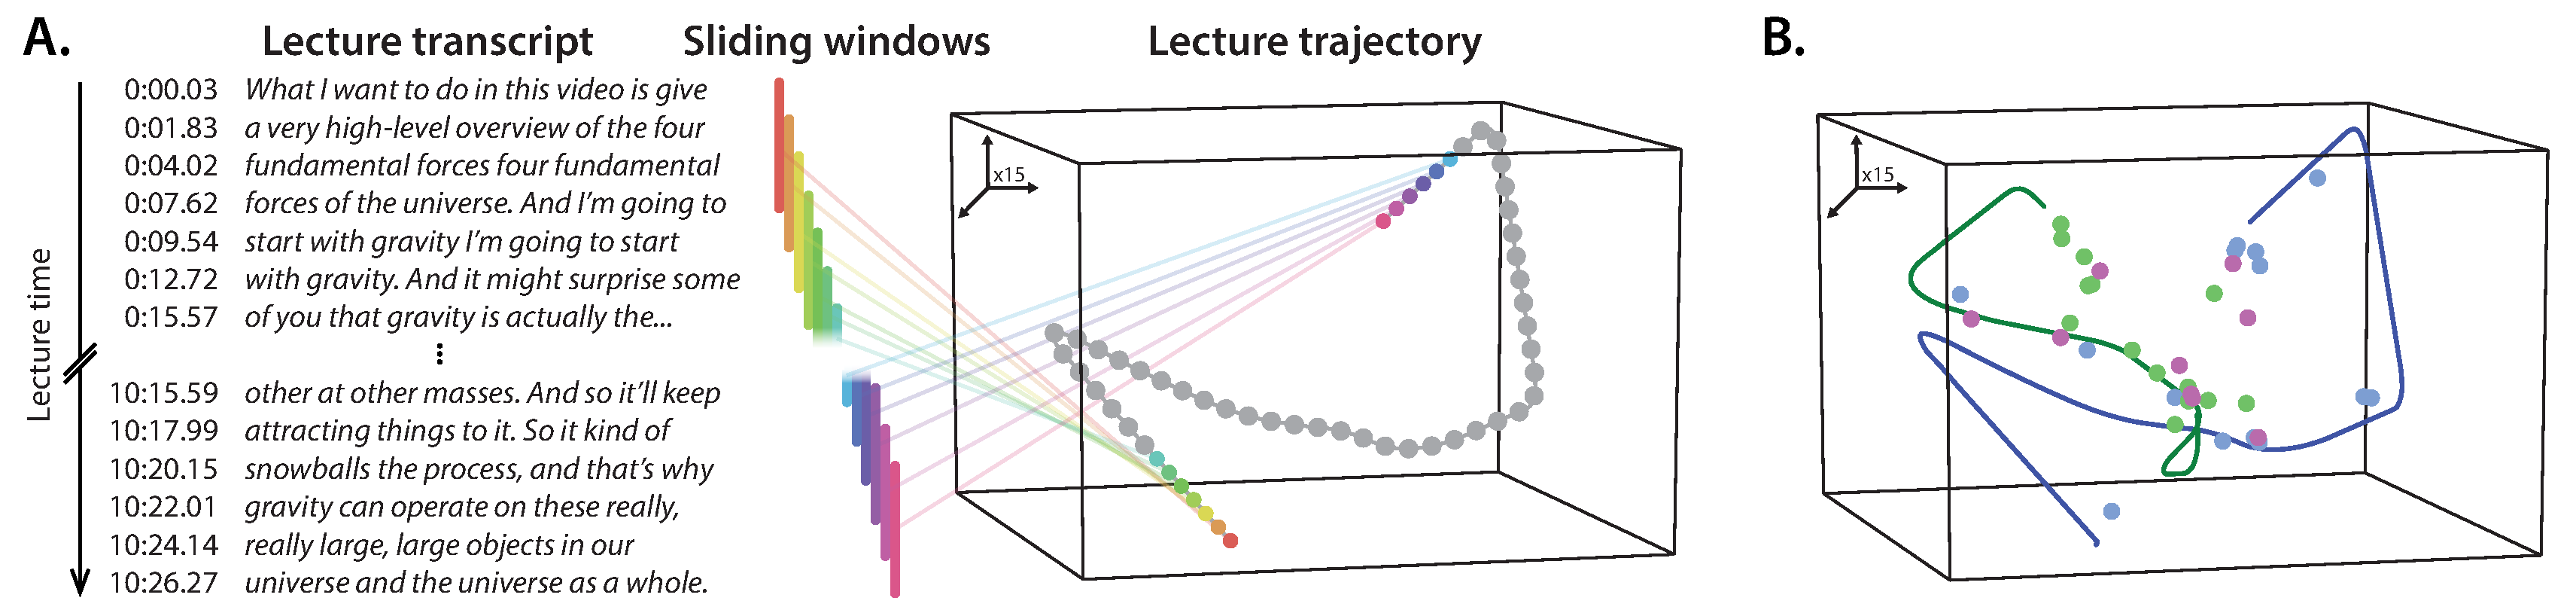
\includegraphics[width=\textwidth]{figs/sliding_windows}

\caption{\textbf{Constructing video content \textit{trajectories}. \textbf{A.
Building a document pool from sliding windows of text.} We decompose each
video's transcript into a series of overlapping sliding windows. The set of
transcript snippets (across all windows) may be treated as a set of
``documents'' for training a text embedding model. After training a text
embedding model using the two videos' sliding windows, along with the text from
each question in our pool (Tab.~\questions), } we construct ``trajectories''
through text embedding space by joining the embedding coordinates of successive
sliding windows from each video. \textbf{B. Embedding multiple videos and
questions.} Applying the same text embedding approach to each video, along with
the text of each question, results in one trajectory per video and one
embedding coordinate (dot) per question (blue: \textit{Four Fundamental
Forces}; green: \textit{Birth of Stars}; pink: general physics knowledge). Here
we have projected the 15-dimensional embeddings into a 3D space using Uniform
Manifold Approximation and Projection~\citep[UMAP;][]{McInEtal18a}.}

\label{fig:sliding-windows}
\end{figure}

As illustrated in Figure~\ref{fig:sliding-windows}A, we start by building up a
corpus of documents using overlapping sliding windows that span each video's
transcript. Khan Academy videos are hosted on the YouTube platform, and all
YouTube videos are run through Google's speech-to-text API~\citep{HalpEtal16}
to derive a timestamped transcript of any detected speech in the video. The
resulting transcripts contain one timestamped row per line, and each line
generally corresponds to a few seconds of spoken content from the video. We
defined a sliding window length of (up to) $w = 30$ transcript lines, and we
assigned each window a timestamp according to the midpoint between its first
and last lines' timestamps. These sliding windows ramped up and down in length
at the very beginning and end of the transcript, respectively. In other words,
the first sliding window covered only the first line from the transcript; the
second sliding window covered the first two lines; and so on. This insured that
each line of the transcript appeared in the same number ($w$) of sliding
windows. We treated the text from each sliding window as a single ``document,''
and we combined these documents across the two videos' windows to create a single
training corpus for the topic model.  The top words from each of the 15 discovered
topics may be found in Table~\topics.

After fitting a topic model to each videos' transcripts, we could use the
trained model to transform arbitrary (potentially new) documents into
$k$-dimensional topic vectors. A convenient property of these topic vectors is
that documents that reflect similar blends of topics (i.e., documents that
reflect similar themes, according to the model) will yield similar (in terms of
Euclidean distance, correlation, etc.) topic vectors. In general, the
similarity between different documents' topic vectors may be used to
characterize the similarity in conceptual content between the documents.

We transformed each sliding window's text into a topic vector, and then used
linear interpolation (independently for each topic dimension) to resample the
resulting timeseries to once per second. This yielded a single topic vector for
each second of each video. We also used the fitted model to obtain topic
vectors for each question in our pool (Tab.~\questions). Taken together, we
obtained a \textit{trajectory} for each video, describing its path through
topic space, and a single coordinate for each question
(Fig.~\ref{fig:sliding-windows}B). Embedding both videos and all of the
questions using a common model enables us to compare the content from different
moments of videos, compare the content across videos, and estimate potential
associations between specific questions and specific moments of video.


\subsubsection*{Estimating dynamic knowledge traces}

We used the following equation to estimate each participant's knowledge about
timepoint $t$ of a given lecture, $\hat{k}(t)$:
\begin{equation}
    \hat{k}\left(f(t, L)\right) = \frac{\sum_{i \in \mathrm{correct}}\mathrm{ncorr}\left(f(t, L), f(i, Q)\right)}{\sum_{j = 1}^N \mathrm{ncorr}\left(f(t, L), f(j, Q)\right)},
    \label{eqn:prop}
\end{equation}
where

\begin{equation}
    \mathrm{ncorr}(x, y) = \frac{\mathrm{corr}(x, y) - \mathrm{mincorr}}{\mathrm{maxcorr} - \mathrm{mincorr}},
\end{equation}
and where $\mathrm{mincorr}$ and $\mathrm{maxcorr}$ are the minimum and maximum
correlations between any lecture timepoint and question, taken over all
timepoints and questions across both lectures and all three question sets. We
also define $f(s, \Omega)$ as the $s$\textsuperscript{th} topic vector from the
set of topic vectors $\Omega$. Here $t$ indexes the set of lecture topic
vectors, $L$, and $i$ and $j$ index the topic vectors of questions in the
quiz's question set, $Q$. Note that ``correct'' denotes the set of indices of
the questions the participant answered correctly on the given quiz.

Intuitively, $\mathrm{ncorr}(x, y)$ is the correlation between two topic
vectors (e.g., the topic vector from one timepoint in a lecture, $x$, and the
topic vector for one question, $y$), normalized by the minimum and maximum
correlations (across all timepoints and questions) to range between 0 and 1,
inclusive. Equation~\ref{eqn:prop} then computes the weighted average
proportion of correctly answered questions about the content presented at
timepoint $t$, where the weights are given by the normalized correlations
between timepoint $t$'s topic vector and the topic vectors for each question.
The normalization step (i.e., using $\mathrm{ncorr}$ instead of the raw
correlations) insures that every question (except the least-relevant question)
contributes some non-zero amount to the knowledge estimate.

\subsubsection*{Creating knowledge and learning map visualizations}

An important feature of our approach is that, given a trained text embedding
model and participants' quiz performance on each question, we can estimate
their knowledge about \textit{any} content expressible by the embedding model--
not solely the content explicitly probed by the quiz questions. To visualize
these estimates
(Figs.~\ref{fig:knowledge-maps},~\individualKnowledgeMapsA,~\individualKnowledgeMapsB,~\individualKnowledgeMapsC,~\individualLearningMapsA,
and~\individualLearningMapsB), we used UMAP~\citep{McInEtal18a} to define a 2D
projection of the text embedding space. Sampling the original 100-dimensional
space at high resolution to obtain an adequate set of topic vectors spanning
the embedding space would be computationally intractable. However, sampling a
2D grid is much more feasible. We defined a rectangle enclosing the 2D
projections of the lectures' and quizzes' embeddings, and we sampled points
from a regular $100 \times 100$ grid of coordinates that evenly tiled the
enclosing rectangle. We sought to estimate participants' knowledge (and
learning---i.e., changes in knowledge) at each of the resulting 10000
coordinates.

To generate our estimates, we placed a set of 39 radial basis functions (RBFs)
throughout the embedding space, centered on the 2D projections for each
question (i.e., we included one RBF for each question). At coordinate $x$, the
value of an RBF centered on a question's coordinate $\mu$, is given by:
\begin{equation}
    \mathrm{RBF}(x, \mu, \lambda) = \exp\left\{-\frac{||x - \mu||^2}{\lambda}\right\}.
    \label{eqn:rbf}
\end{equation}
The $\lambda$ term in the RBF equation controls the ``smoothness'' of the
function, where larger values of $\lambda$ result in smoother maps. In our
implementation we used $\lambda = 50$.  Next, we estimated the ``knowledge''
at each coordinate, $x$, using:
\begin{equation}
    \hat{k}(x) = \frac{\sum_{i \in \mathrm{correct}} \mathrm{RBF}(x, q_i, \lambda)}{\sum_{j = 1}^N \mathrm{RBF}(x, q_j, \lambda)}.
    \label{eqn:rbf-knowledge}
\end{equation}
Intuitively, Equation~\ref{eqn:rbf-knowledge} computes the weighted proportion of
correctly answered questions, where the weights are given by how nearby (in the 2D space)
each question is to the $x$.  We also defined \textit{learning maps} as the coordinate-by-coordinate
differences between any pair of knowledge maps.  Intuitively, learning maps reflect the \textit{change}
in knowledge across two maps.

\section*{Author contributions}

Conceptualization: PCF, ACH, and JRM. Methodology: PCF, ACH, and JRM. Software:
PCF. Validation: PCF. Formal analysis: PCF. Resources: PCF, ACH, and JRM. Data
curation: PCF. Writing (original draft): JRM. Writing (review and editing):
PCF, ACH, and JRM. Visualization: PCH and JRM. Supervision: JRM. Project
administration: PCH. Funding acquisition: JRM.


\section*{Data and code availability}

All of the data analyzed in this manuscript, along with all of the code for
running our experiment and carrying out the analyses may be found at
https://github.com/Con\-text\-Lab/eff\-ic\-ient-learn\-ing-khan.

\section*{Acknowledgements}

We acknowledge useful discussions, assistance in setting up an earlier
(unpublished) version of this study, and assistance with some of the data
collection efforts from Will Baxley, Max Bluestone, Daniel Carstensen, Kunal
Jha, Caroline Lee, Lucy Owen, Xinming Xu, and Kirsten Ziman. Our work was
supported in part by NSF CAREER Award Number 2145172 to JRM. The content is
solely the responsibility of the authors and does not necessarily represent the
official views of our supporting organizations. The funders had no role in
study design, data collection and analysis, decision to publish, or preparation
of the manuscript.



\bibliographystyle{apa}
\bibliography{CDL-bibliography/cdl}
\end{document}
